\documentclass[aasms,12pt]{article}
\usepackage{natbib}
\setlength{\bibsep}{0pt plus 0.3ex}
\usepackage{sectsty}
\usepackage{graphicx}
\usepackage[skip=2pt,font=small]{caption}
\captionsetup{width=\textwidth}


\sectionfont{\normalsize}
\usepackage{fullpage}

%\usepackage[margin=1in]{geometry}

%\citestyle{aa}
\newcommand{\sol}{\ensuremath{\odot}}


\usepackage{fancyhdr}
\pagestyle{fancy}
\fancyhf{} % sets both header and footer to nothing
\renewcommand{\headrulewidth}{0pt}
\cfoot{\thepage}
\rfoot{\footnotesize{Evan Anders, NASA NESSF 2015}}




\begin{document}
\begin{center}
   \large\textbf{The solar dynamo: Understanding the tachocline's role and bridging
	the gap between simulation and observation}\\
   \vspace{0.4cm}
   \large{Evan Anders}\\
   \vspace{0.4cm}
   \normalsize\textit{Advisor: Benjamin Brown}\\
   \normalsize\textit{LASP, University of Colorado at Boulder}\\
\end{center}



\abstract{The Sun is magnetically active due to a magnetic dynamo
	powered by the solar convective zone.  Numerical simulations have
	offered great insight into the nature of the magnetic fields intrinsic
	to this dynamo.  Traditionally, these simulations
	are carried out for solar-type stars with high rotation rates
	and characteristic convective motions much larger than those realisable
	within the Sun.  Here I propose to create a
	suite of 3-D numerical simulations of the solar convective zone
	with accurate solar rotation and convective velocity profiles.  
	My primary
	goal is to determine the role of the solar tachocline, the rotational
	shear layer at the base of the convective zone, in producing
	and sustaining the solar magnetic dynamo.  Furthermore, a more
	detailed set of simulations which include the supergranulation of
	the solar photosphere will be created and post-processed to create
	synthetic observable which will be directly comparable with 
	data such as that gathered the Solar Dynamics Observatory and other
	spacecraft.}



\section{Introduction}
The Sun is a magneticly active star.  Its magnetism arises from an 
organized dynamo seated in the turbulent plasma
motions of the solar convective zone, which occupies roughly the outer 30\%
of the Sun's radius.  In the presence of
convective motions, magnetic fields and solar rotation couple to produce global
wreaths of magnetism which drive the Sun's 22-year cycle of magnetic activity.
This activity manifests itself in the collection of phenomena which is generally
referred to as solar activity, including magnetic storms and coronal mass
ejections.  Such activity propagates towards Earth, threatening disruption power
grids and aircraft operations and endangering astronauts and satellites.  It is
clear that the Sun's magnetism affects our increasingly technological society;
understanding the nature of the dynamo that drives solar magnetism is of
paramount importance.

While current simulations lack the power to accurately 
predict the stellar magnetic environment 
over long time scales, they have provided great insight into the mechanisms
underlying the solar dynamo over the past decade.  
It has 
Observationally, it is known that the surface of the sun rotates differentially,
with the poles rotating roughly every 35 days and the equator rotating every 25
days.
Through probing the Sun's
radial structure and sub-surface convective flows using acoustic oscillations,
helioseismology
has revealed that the solar differential rotation profile extends through the
bulk of the convective zone with two distinct shear regions.  A near-surface
shear layer occupies roughly the outer 5\% of the Sun and a secondary shear
layer, called the tachocline, resides at the base of the convective zone
and separates the differentially rotating convective zone from the uniformly
rotating radiative zone located radially inward.  
Traditional models of the solar dynamo, namely Babcock-Leighton flux-transport
dynamo models and interface dynamo models, have stated that the
tachocline drives the production of the toroidal magnetic   
fields which fuel the solar dynamo and manifest at the solar surface as
sunspots (\citealt{Toomre2009}).  In such models, magnetic fields generated
in the convective zone are transported inward to the tachocline, where
magnetic wreaths are built before buoyantly 
rising to the solar surface.

Numerically simulating the solar environment requires working with wide ranges
of spatial and temporal timescales, which is one of the main sources of
difficulty in creating meaningful simualtions.  Regardless of this, the
underlying equations at the heart of these magnetohydrodynamic (MHD) simulations
are quite simple, expressing conservation of mass, momentum, and energy and
accounting for magnetic induction (\citealt{Charbonneau2014}).  Most simulations
have modelled stars with higher rotation rates than the sun, as the strength
of the magnetic dynamo increases with increasing rotation rate (see Fig.
\ref{wreaths}a).  Such simulations
have largely informed solar dynamo theory and have even generated 
self-sustaining, buoyantly-rising toroidal wreaths of magnetism with polarity
shifts on long time scales,
such as those shown in Fig. \ref{wreaths}b\&c.  

In the context of accepted dynamo theory, an unsettling result has arisen
in recent simulations of Sun-like stars: there is a disagreement
regarding the necessity of the tachocline
in sustaining the solar magnetic dynamo.  Stable solar dynamos have been
created in 3-D numerical simulations both with
(\citealt{ghizaru2010, racine2011})
and without (\citealt{brown2011, nelson2013}) the presence of a tachocline. This
begs the fundamental question: is the tachocline a necessary ingredient in the
production of the solar toroidal magnetic field?  Furthermore, is a tachocline
necessary to produce a solar dynamo?  Those simulations which produced opposing
results were made with different codes using differing models for subgrid
processes at various stellar rotation rates.  Consequently, it is impossible to
meaningfully compare the results of the simulations directly.  The data required
to determine the necessity and role of the tachocline are missing.

Additionally, most simulations
of solar convection simulate Sun-\emph{like} stars rather than the Sun
itself.  Such simulations model starts with greater rotation rates and greater
convective flow velocities than our sun.  It has recently been discovered
that these simulations may not accurately capture the physics at work
in the Sun as they assume much larger amplitudes of large scale convective
motions than those that are actually present in the Sun
(\citealt{lord2014}).  Such a discovery calls for a new set of solar 
numerical simulations with a more accurate description of convective flows
than that which has existed in previous simulations.

Through lowering the stellar rotation rate to that of the solar rotation rate
and decreasing the amplitudes of convective motions within modeled solar
convection zones, it is now possible to gain an understanding of the physics at
work within the Sun itself through simulations, rather than just sun-like
stars.
Furthermore, while simulations of stellar magnetic dynamos have proven
irreplaceable in gaining insight into the structure and evolution of 
long-term cycles, they fail to compare to \emph{in-situ} measurements
of solar magnetism and cannot provide insight on short-term scales.
With the wealth of spacecraft currently gathering data on
the Sun in addition to the numerous missions which are scheduled to launch
within the next decade, now is the time to bridge the gap between theoretical
dynamo simulations and direct observations of solar activity.


\begin{figure}[t!]
\centering
\includegraphics[width=14cm]{figs/Pizzolato_and_D5.eps}
\caption{(a) Observationally determined relations between magnitude of stellar
	x-ray luminosity versus rotation period showing a clear increase in
	x-ray luminosity (powered by stellar magnetism) with decreasing rotation
	periods (\citealt{Pizzolato2003}).  (b) Toroidal wreaths of magnetism
	obtained through numerical simulations with the ASH code which show a
	clear polarity inversion (c) over long time scales.
        \label{wreaths}}
\end{figure}


\section{Does the tachocline drive the sun's toroidal magnetic fields?}
I propose a set of hydrodynamical simulations of the Sun's convective zone
which test the role of a tachocline in the generation of a solar magnetic 
dynamo.  These simulations will model the majority of the solar convective
zone, from its base around $R = 0.713R_{\odot}$ up into the base of the outer
shear layer, stopping
around $R = 0.97R_{\odot}$.  These simulations will include identical rotation
rates and convective timescales, but one simulation will include the shear
effects of the tachocline and one simulation will not.
As dynamo theory champions the tachocline as the seat of the toroidal component
of the solar magnetic field, it is time to put this theory to the test.
The likeness of these simulations will allow for a direct comparison of their
results, allowing a certainty regarding the role---or lack thereof---of the
tachocline in generating and maintaining the solar dynamo.

I will use the widely-known Anelastic Spherical Harmonic (ASH, 
\citealt{clune1999}) spectral solver, which I will have access to through my
advisor, Ben Brown, to create my simulations.  The use of a well-established
code such as ASH will allow me to
efficiently model the solar convective zone in spherical coordinates and gain
and understanding of the physics driving the solar dynamo without having to
worry about generating a fully functional modelling suite.  Naturally, work
of this magnitude requires access to massively parallel computing resources.
As a CU Boulder student, I have access to the school's local supercomputer,
\emph{Janus}.  Additionally, I will work with Ben Brown to acquire CPU time on
state-of-the art supercomputers such as the NSF XSEDE resources and NASA's
\emph{Pleiades}. 

I have been well prepared by my past education to undertake the creation of
a simulation of this magnitude.  
In 2012, I worked with
Pacific Northwest National Laboratory's (PNNL) Data Intensive Scientific
Computing group and gained an understanding of the challenges faced in the
creation of large, scientific computations.  In addition to learning the
struggles faced in efficiently creating massively parallelised algorithms,
I learned how to effectively understand and utilize computational tools
(such as ASH) created by others for my own purposes. Furthermore, I learned
numerous techniques for debugging and optimizing my routines.

Furthermore, over the summer of 2013, I participated in the NSF Science
Undergraduate Research Fellowship program at the Laser Interferometer
Gravitational-wave Observatory (LIGO).  During my time at LIGO Hanford, it was
my task to create a computational tool which analyzed LIGO science run data at
specific frequencies and output information about the data at those frequencies
in user-friendly text files.  This experience taught me how to interact with
massive quantities of data, how to organize that data meaningfully in files,
and how to effectively plot and visualize such data.  All of these skills
will be exceptionally useful at all stages in massive 3D simulations.

Coupled with my strong undergraduate education in physics, I am in the process
of learning the fundamentals of fluid mechanics and plasma physics necessary to
understand and implement the processes which govern the motion of the solar 
convective zone.

\section{Simulated observables: Connecting observations and simulations}
While simulations are extremely beneficial in gaining an understanding of the
physical trends occuring within a system, they often fall short of a direct
connection to observable data.  Thus, I propose a second suite of simulations:
one which spans the entirety of the solar convective zone and reaches out to
the solar photosphere in order to determine the behavior of the magnetic fields
at the observable surface of the Sun.  In efforts to model the true physics of
the Sun as acurately as possible, these simulations will capture supergranular 
scales but will ignore small scale granulation.  This simplification will be
made for two reasons.  First, the small scale motion of granulation is unlikely
to greatly affect the overall motions of the vast solar convective zone (as
they have characteristic length scales roughly two orders of magnitude apart).
Second, the computational load that would be required to resolve granular scales
would push the number of CPU hours required for a project of this magnitude
past that which is feasible to acquire on state-of-the-art machines.

Numerous post-processing techniques would be used on the photospheric data 
given by these simulations in order to create synthetic observables.
Atmospheric and radiative transfer models would be used to transform simulation
data (which is known precisely in terms of fields and velocities) into
observable phenomena (namely, sunspots). 
Presumably, simulations
which accurately capture the physics at work within the solar convective zone
will create patterns similar to those observed at the solar surface.  If
simulated sunspots behave similarly to real sunspots, then we know that our
theory of the dynamo is working properly and we will have taken a step towards
being able to predict solar weather through pattern recognition.

The synthetic observables created by these simulations would be directly
comparable to data from the Solar Dynamics Observatory (SDO) and the Van Allen
Probes.  Those structures and behavioral patterns which arise in the results
of the proposed simulations can offer insights into the workings of the real
solar convective zone and can potentially be used to predict unusual solar
activity in the future.  Furthermore, the scheduled Solar Orbiter Collaboration
(SCO) will be the first spacecraft to study the solar poles in detail.  While
current spacecraft will prove beneficial in drawing ties between theoretical
structure and actual magnetic structures near the solar equator, SCO will offer
an opportunity to understand the results of such simulations along the solar
poles. 

\begin{figure}[t!]
\centering
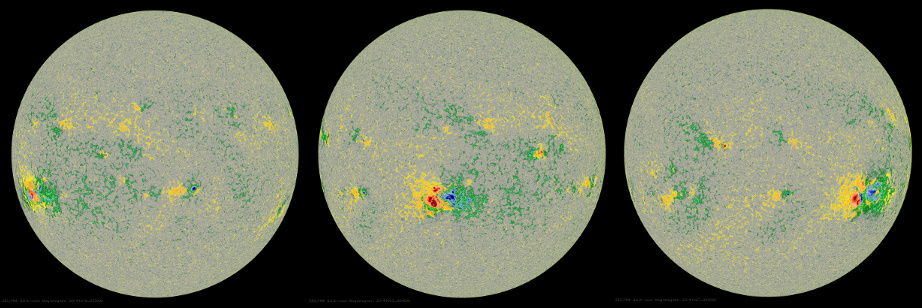
\includegraphics[width=14cm]{figs/2014_oct_sunspots.jpg}
\caption{SDO Colorized magnetogram images of solar active region AR 12192, taken
	on 10/19/2014, 10/23/2014, and 10/27/2014, respectively.  Simulated
	observables could mimic the behavior of regions such as this and help
	us understand when and why they release solar flares such as the X3.1
	flare released on 10/24/2014.
	\label{AR12192}}
\end{figure}

\section{Relevance to NASA} 
The proposed work fits perfectly with NASA's 2014 Strategic plan objectives
1.4:
``Understand the Sun and its interactions with Earth and the solar
system, including space weather.''
This work also fits in with one of the three overarching science goals
of the Heliophysics section of NASA's 2014 Science plan: 
``Develop the
knowledge and capability to detect and predict extreme conditions in space to
protect life and society and to safeguard human and robotic explorers beyond
earth.''

In order to predict extreme space conditions caused by the Sun's magnetic
activity, we must have an intricate understanding of the behavior of the Sun's
magnetic dynamo.  While solar dynamo theory has progressed impressively over
recent years, it has progressed with an untested assumption as a cornerstone
and a series of impressive simulations with no tangible connection to
observables.  After recent simulations have disagreed regading the importance
of the tachocline in the production of the solar magnetic dynamo, it is time
to put the assumed importance of the tachocline to the test.  Furthermore,
it is time to connect simulations to the real world.  In order to have a
consistent, predictive theory on the behavior of the solar magnetic field, it
is necessary to connect theoretical calculations---those largely present in
large-scale numerical simulations---with tangible observables.  Only once these
two sources of data are connected will we be able to possibly predict upcoming
solar magnetic behavior.



\nocite{*}
\bibliographystyle{apj}
\begingroup
\renewcommand{\section}[2]{}%
\begin{footnotesize}
\bibliography{biblio}
\end{footnotesize}
\endgroup
\end{document}
